
% The \phantomsection command is needed to create a link to a place in the document that is not a
% figure, equation, table, section, subsection, chapter, etc.
% https://tex.stackexchange.com/questions/44088/when-do-i-need-to-invoke-phantomsection
\phantomsection

\chapter{Evaluation of Primal Heuristics}\label{chap:evaluation}

As discussed in Chapter\,\ref{chap:integer-programming}, Section\,\ref{sec:heuristics}, a primal heuristic abides from optimality guarantees to focus on a trade-off between solution quality and computational cost (speed).
Consequently, two primal heuristics for MILP problems can be compared with respect to how fast they provide solutions and how good they are, and whether the solutions are feasible or not.
% In this chapter, two approaches are discussed to evaluate primal heuristics.
In this chapter, multiple metrics are presented to cover the two perspectives in which a heuristic can be said superior to another.
% The first (Sec.~\ref{sec:standard-evaluation-metrics}) is based on standard evaluation metrics. Therefore, it uses multiple metrics, one for each
% The second (Sec.\,\ref{sec:primal-integral}) is specific to primal heuristics that improve the candidate solution over time, such as matheuristics.
% By tracing the progress of the candidate solution, it provides a single metric that takes into account the characteristic trade-off of primal heuristics.

% - como discutido na sec XXX, ao abrir mão da garantia de otimalidade, uma heurística primal oferece a possibilidade de trocar qualidade da solução por velocidade de otimização.
% - nesse sentido, duas heurísticas podem ser comparadas em função dessa relação
% - neste capítulo, duas abordagens serão apresentadas para caracterizar a qualidade de heurísticas. a primeira, através de múltiplas métricas que são comumente para avaliar qualquer tipo de heurística
% - a segunda, específica para matheuristics, que explora a sua característica de aprimorar a solução candidata ao longo do tempo

% \phantomsection
\section*{}
% \section{Standard Evaluation Metrics}\label{sec:standard-evaluation-metrics}

The objective value and the time taken to provide a solution are natural evaluation metrics.
However, they have significant shortcomings.
The value of the cost function (supposing a minimization problem) is hard to interpret without bounds.
For example, it is difficult to judge how better one heuristic approach is with respect to the other just by knowing that the first provided a solution with a cost of 10, while the second provided a solution with a cost of 15.
If the optimal solution costs -1000 and a trivial solution costs 20, then it can be said that both heuristics performed poorly.
On the other hand, if the optimal solution has a cost of 9 and a trivial solution has cost 15, then it can be said that the first heuristic performed much better than the second.

Therefore, to make a fair judgment about the solution quality of a set of heuristics being evaluated, one needs to know both the cost of the solutions as well as upper and lower bounds for the problem.
Beyond the difficulty of determining such bounds, having a multidimensional metric for judging solution quality can make it more challenging to compare the performance across different optimization problems and even across different instances of the same problem.
An alternative to summarizing all these values is to compute the cost of the heuristic solution normalized between the optimal cost (0~\%) and the cost of the trivial solution (100~\%).
Let $\hat{\bm{y}}$ be a heuristic solution, $\bm{y}^*$ be the optimal solution, and $\overline{\bm{y}}$ be a trivial solution for an instance of an optimization problem as in \eqref{eq:general-milp}.
Then, \emph{relative cost} of $\hat{\bm{y}}$ can be defined as
\begin{equation}
    \text{RelCost}(\hat{\bm{y}}) = \frac{\bm{c}^{T} \hat{\bm{y}} - \bm{c}^{T} \bm{y}^*}{\bm{c}^{T}\overline{\bm{y}} - \bm{c}^{T}\bm{y}^*}
.\end{equation}

Similarly, if the problem of interest is a maximization problem, then one can define the \emph{relative objective} of a candidate solution $\hat{\bm{y}}$ as
\begin{equation}\label{eq:relobj}
    \text{RelObj}(\hat{\bm{y}}) = \frac{\bm{c}^{T} \hat{\bm{y}}  - \bm{c}^{T}\overline{\bm{y}}}{\bm{c}^{T}\bm{y}^* - \bm{c}^{T}\overline{\bm{y}}}
.\end{equation}

Certain conditions must be met to evaluate an approach's efficiency, ensuring that the time taken to compute a solution (runtime) is meaningful and fair.
One way to do so is to ensure that the computational resources are fairly available to all approaches.
Usually, this implies in allowing all approaches to have plain access to a common hardware, i.e., that there are no other processes using the resources during the time of execution.

Still, there are a few caveats in this performance metric, of which parallelization abilities are probably the most prominent.
Comparing single-process with multi-process approaches is quite difficult, as a process that can compute its results in parallel uses more resources in the same runtime. 
Furthermore, projecting empirical results to different setups is challenging when the processes being evaluated use parallel computation. 
% An alternative would be to compute the total computational time, e.g., if a process is running 
In this work, it is considered that parallelization is commonly supported in modern hardware configurations.
Thus, the runtime is computed as the user-perceived real time (or wall time) for the heuristic to provide a solution given an instance of an optimization problem, regardless of whether parallelization was used or not.

% \section{The Primal integral}\label{sec:primal-integral}

% % see https://www.ecole.ai/2021/ml4co-competition/#metrics

% Although relative cost can be used to compare heuristics given a fixed time budget, it does not properly suit the cases where the time taken by a heuristic has a variable cost.
% For such cases, it is possible to use the integral of the relative cost over time, or the \emph{primal integral}, as used in \citeonline{gasseMachineLearningCombinatorial2022}.
% To see this, consider a heuristic that provides increasingly better solutions over time.
% One could define the cost at time $t$ as the cost associated with the best solution up to time $t$.
% Figure~\ref{fig:primal-curve} illustrates the evolution of the cost over time (orange curve).
% The primal integral is precisely the integral of such cost over time, which can be written \[
%     \int \bm{c}^T \hat{\bm{y}}(t) dt
% ,\] where $\hat{\bm{y}}(t)$ is the best solution known (or candidate solution) at time $t$.
% It is called the primal integral because it computes the integral of the cost associated with primal solutions.

% \begin{figure}[h]
%     \centering
%     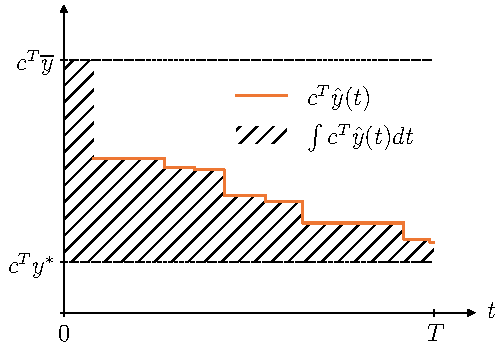
\includegraphics{primal.pdf}
%     \caption{Example of primal integral computation. $y^*$ and $\overline{y}$ are (sub-)optimal and trivial solutions, respectively. The orange curve represents the evolution of the candidate solution's cost over time. Note that the orange curve is not defined at the beginning of the runtime, indicating that a candidate solution is not provided at $t=0$. The hatched area is the primal integral, bounded by the two references ($y^*$ and $\overline{y}$).}
%     \label{fig:primal-curve}
% \end{figure}

% The straightforward integral of the primal curve, however, has two major limitations.
% First, it is not properly defined at $t \to 0$, as it is not expected that a heuristic starts with a candidate solution, i.e., $\hat{y}(0)$ is not defined.
% Furthermore, the length of this undefined region varies from heuristic to heuristic, which hinders fair comparisons.
% One way to circumvent this problem is to assume that $\hat{\bm{y}}(t) = \infty$ before the first candidate solution is provided, and compute the integral of the minimum between $\bm{c}^T \hat{\bm{y}}$ and $\bm{c}^T\overline{\bm{y}}$ (the cost of a trivial solution).
% This way, a heuristic approach is penalized for taking longer to provide a candidate solution.

% The second limitation is that the result is not comparable across different instances of a problem.
% This is because the cost of a candidate solution is meaningless, unless it is necessary to understand how close to the optimal and how far from trivial that given solution is.
% One way to attenuate this problem is to normalize the integral with respect to the difference between the cost of the trivial solution and the cost of the optimal solution.
% This approach can be interpreted as normalizing the integrals with respect to the integral of the naïve heuristic, which is simply to guess the trivial solution.

% In summary, the practical primal integral of a heuristic $H$ that can provide candidate solutions over time $\hat{\bm{y}}_H(t)$ is defined as
% \begin{equation}\label{eq:primal-integral}
%     \text{PrimalIntegral}(H) = \frac{1}{T(\bm{c}^T \overline{\bm{y}} - \bm{c}^T \bm{y}^*)} \int_0^{T} \left( \min\left( \bm{c}^T \overline{\bm{y}}, \bm{c}^{T} \hat{\bm{y}}_H(t) \right)  - \bm{c}^{T} \bm{y}^* \right)  dt
% ,\end{equation}
% where $\overline{\bm{y}}$ is a trivial solution and $\bm{y}^*$ is an optimal solution.
% Such is illustrated in Fig.~\ref{fig:primal-curve} through the hatched region.

